\documentclass[12pt, a4paper]{article}
\usepackage[utf8]{inputenc}
\usepackage{amsmath}
\usepackage{amsfonts}
\usepackage{amsthm}
\usepackage{array}
\usepackage{graphicx}
\usepackage{parskip}
\usepackage[pdfencoding=auto]{hyperref}
\usepackage{fancyhdr}
\usepackage{lastpage}
\usepackage{tikz}
\usepackage{float}
\usepackage{listings}
\usepackage{color}
\usepackage{caption}
\usepackage[acronym]{glossaries}
\usepackage[nottoc]{tocbibind}
\usepackage[cache=false]{minted}
\usemintedstyle{default}
\newminted{haskell}{frame=lines,framerule=2pt}
\graphicspath{{./images/}}

\tikzstyle{bag} = [align=center]

\title{%
      Final Homework\\
      Analysis of Random Access Zippers
}
\author{%
  Juan Pablo Royo Sales \\
  \small{Universitat Politècnica de Catalunya}
}
\date\today

\pagestyle{fancy}
\fancyhf{}
\fancyhead[C]{}
\fancyhead[R]{Juan Pablo Royo Sales - UPC MIRI}
\fancyhead[L]{ADS - Final Homework}
\fancyfoot[L,C]{}
\fancyfoot[R]{Page \thepage{} of \pageref{LastPage}}
\setlength{\headheight}{15pt}
\renewcommand{\headrulewidth}{0.4pt}
\renewcommand{\footrulewidth}{0.4pt}

\newacronym{haskell}{Haskell}{Haskell Programming Language}
\newacronym{kde}{KDE}{Kernel Density Estimate}
\newacronym{lrm}{LRM}{Linear Regression Model}
\newacronym{raz}{RAZ}{Random Access Zippers}
\newacronym{zip}{Zipper}{Zipper}
\newacronym{pbbt}{PBBT}{Probabilistic-Balanced Binary Tree}
\newacronym{ftree}{F-Tree}{Finger Trees}
\newacronym{rrb-v}{RRB-Vector}{RRB-Vector}
\newacronym{bst}{BST}{Binary Search Trees}
\newacronym{fp}{FP}{Functional Programming}
\newacronym{ocaml}{OCaml}{OCaml Programming Language}
\newacronym{nbd}{NBD}{Negative Binomial Distribution}

\begin{document}

\maketitle

\section{Introduction}\label{sec:intro}
The propose of this work is to Analyzed and reproduced the work and experiments of \textbf{\acrfull{raz}} written for the first time here \cite{raz}. Additionally the original work has been done with \acrfull{ocaml} and the idea of this work was to first give an efficient \acrfull{haskell} implementation and secondly using that implementation reproduced the experiments.

This translations might not seen so obvious for the unexperienced reader but because of \acrshort{ocaml} nature which has \textbf{Strict evaluation} by default compared with \acrshort{haskell} that has \textbf{Non Strict} one, things cannot be translate one to one always.

\textbf{\acrfull{raz}} is a combination of a \textbf{\acrfull{zip}} Data Structure with a simple \acrfull{bst}, in fact with a \textbf{\acrfull{pbbt}}. This powerful combination enables to have a \textit{Sequence} like structure with $O(1)$ edit time and $O(\log{n})$ amortized time for random access elements.

In the following sections I am going to describe:

\begin{itemize}
 \item Brief introduction of the Structure and its main features
 \item Implementation Details
 \item Experiments that have been reproduced from the paper plus other additional experiments
 \item Conclusions
\end{itemize}

\section{Asset organization}
Please check the appendix~\ref{apx:org} to see how the different assets are organized, how to run the experiment, and so on.

\section{Analysis of RAZ's paper}
\subsection{Motivation}
The motivation of this data structure appears with the intention to have an \textbf{\textit{purely functional Sequence}} like data structure with better performance on edition and random access in worst case and amortized case, because typical sequence structures in \acrfull{fp} world, \textit{List}, has only efficient edit and access on the \textit{head} of the list, but requires \textbf{linear} time on worst case.

It is well known as it is stated on the paper that there were \textbf{2(two) other} data structures, \acrfull{ftree} and \acrfull{rrb-v} most recently, that overcome this issues in \acrshort{fp} sequence like. But the implementation of this 2 data structures are complex and not so extensible as \textit{List}. \acrshort{raz} main motivation is to give the same performance as \acrshort{ftree} and \acrshort{rrb-v} with the simplicity for extension as \textit{Lists}.

\subsection{Structure brief summary}\label{sub:sec:1}
As I have described, \acrshort{raz} represents a \textit{Sequence} with 2 main data structures, \acrshort{zip} and \acrshort{pbbt}. In order to edit sequences in a \acrshort{fp} Persistent setting, \acrshort{zip} gives the power of \textbf{\textit{cursor}} to focus in some particular position in the sequence. The idea is that this \textit{cursor} positions near the element to be edited, removed or inserted.

This \textit{cursor} is allowed to be moved through the structure interface functions either Right or Left, just as a regular \acrshort{zip}, or in a global manner providing the position where we want to position to. This last is achieve by \acrshort{pbbt} which gives $\log{n}$ time for position globally on any place.

\acrshort{pbbt} is built using a \acrfull{nbd} which yields expected small numbers for levels in the tree allowing to build a balanced tree on the structure. This technique is explained in detailed here \cite{pbbt}.

Basically \acrshort{raz} is built with 3 structures, the \textit{zip} which allowed us to move the cursor, \textit{tree} which allowed us to maintain a balanced structure of all the nodes for fast positioned in a random access manner and \textit{tlist} which is an ordinary \acrshort{fp} list like structure which its \textit{Cons} type holds the \textbf{levels} and the \textbf{trees}. I am going to show in detailed this structure in implementation section~\ref{sec:impl}


\begin{minipage}[t]{\linewidth}
  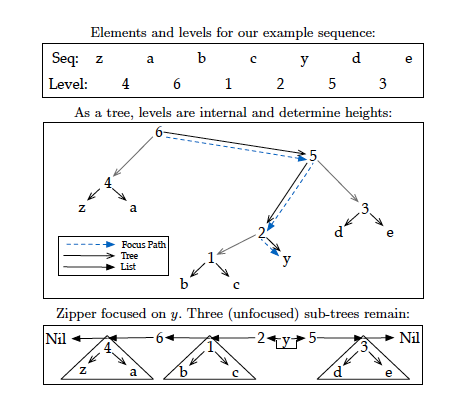
\includegraphics[width=\textwidth]{raz_1}
  \captionsetup{type=figure}
  \captionof{figure}{Raz Structure Example taken from \cite{raz}}
  \label{fig:raz_1}
\end{minipage}

As we can see from the image~\ref{fig:raz_1} giving a sequence, a \acrshort{pbbt} is built with low levels of depths, and focusing in one element like in the example \textbf{\textit{y}} the structure is shaped as a linked list with sub tress at sides.

\subsection{Features and Performance}\label{sub:sec:2}
The following is a copy of the table taken from \cite{raz} where the author's claimed that these are the complexity time requires for each of its main features.

\begin{table}[H]
 \begin{tabular}{|l|l|}
  \hline
   Function:: Type & Time Complexity\\
  \hline
  \mintinline{haskell}{focus :: Int -> Tree a -> Raz a} & $O(\log{n})$ expected \\
  \mintinline{haskell}{unfocus :: Raz a -> Tree a} & $O(\log{n} + m \times \log^2{m})$ expected \\
  \hline
  \multicolumn{1}{|p{3cm}|}{\setlength{\rightskip}{0pt plus 1 fill}\mintinline[breaklines]{haskell}{insert :: RandomGen g => g -> Dir -> a -> Raz a -> (Raz a, g)}} & $O(1)$ worst-case \\
  \hline
  \mintinline{haskell}{remove :: Dir -> Raz a -> Raz a} & $O(1)$ amortized  \\
  \mintinline{haskell}{replaceC :: a -> Raz a -> Raz a} & $O(1)$ worst-case  \\
  \mintinline{haskell}{move :: Dir -> Raz a -> Raz a} & $O(1)$ amortized  \\
  \mintinline{haskell}{viewC :: Raz a -> a} & $O(1)$ worst-case  \\
  \hline
 \end{tabular}
\caption{Main combinators and time complexity}
\label{table:1}
\end{table}

\textbf{\textit{Disclaimer:}} In the author's work \cite{raz} there is any rigorous mathematical analysis on any of this functions and their Time complexity bounds the author's claim.

 \subsubsection{%
 \texorpdfstring{\mintinline{haskell}{focus}}%
  {-{}-enable-so-version}}

  This function allow the user to position globally in a particular element by its index, returning the \mintinline{haskell}{Raz} Type which is the linked list described in the previous section. The authors claimed that this takes $O(\log{n})$ on expectation given a \textit{tree} with depth $d$. This combinator and \mintinline{haskell}{unfocus} analysis is on expected time because it use the \acrshort{pbbt} structure which is based on a probabilistic structure. Although the mathematical analysis of this time is not done by the authors on the paper, it is already proved that a \textit{Balanced Binary Tree} has depth $\log{n}$ as in fact I have done in my first homework on \textit{Randomized Binary Search Trees}, and therefore search will be $O(d)$ where $d$ is the depth of the tree.

 \subsubsection{%
 \texorpdfstring{\mintinline{haskell}{unfocus}}%
  {-{}-enable-so-version}}

 This function allows the opposite of \mintinline{haskell}{focus} which is going back to the \mintinline{haskell}{Tree} \acrshort{pbbt} structure.
 Although as i put in the disclaimer there is no rigorous analysis, in this case the authors go a little deeper in the details.

 As it is described in the table this process by itself takes $O(\log{n} + m \times \log^2{m})$ where $n$ is the length of the sequence and $m$ is the number of \textit{zipped} edits since last refocusing. If $m$ is small the complexity approximates to $O(\log{n})$, but if $m$ grows \acrshort{raz} performs poorly approximating to $O(\log^2{m})$. So to have $m$ small the user needs to do frequents \textit{refocus}. This can be shown by the following prove.

 Given $d$ as the depth of the trees created for the function \mintinline{haskell}{grow} which is an internal operation to build left and right tree, \mintinline{haskell}{grow} requires $O(d)$ time to build the trees. This function also make $d$ calls to \mintinline{haskell}{append} which takes $d$ time also, giving us $O(d^2)$. But since the trees were already put by \mintinline{haskell}{focus}, \mintinline{haskell}{append} takes $O(1)$ amortized. Therefore it takes in total $O(d)$ instead of $d^2$. Since none of this steps dominates asymptotically, composed operations run in $O(d) \sim O(\log{n})$.

 \subsubsection{%
 \texorpdfstring{\mintinline{haskell}{remove}}%
 {-{}-enable-so-version}}

 This function takes constant time amortized, because it implies decomposing the structure in subtrees on $\log{n}$ time, therefore it is constant amortized because of the \textit{edits} that requires.


 \subsubsection{%
 \texorpdfstring{\mintinline{haskell}{move}}%
 {-{}-enable-so-version}}

 This function moves one position on the desire direction, left or right. It uses amortized analysis with the same concept as \mintinline{haskell}{remove} function.

\subsubsection{%
 \texorpdfstring{\mintinline{haskell}{insert}}%
 {-{}-enable-so-version}}

 In this case \mintinline{haskell}{RandomGen} constraint it is because we need to generate the probabilistic level to insert the element to using the \acrshort{nbd}.

 Time complexity is trivial $O(1)$ worst-time because it is focus next to the position to insert the element into.

\subsubsection{%
 \texorpdfstring{\mintinline{haskell}{replaceC}}%
 {-{}-enable-so-version}}

 This is trivial $O(1)$ worst-time because it is focus on the element to be replace with.

\subsubsection{%
 \texorpdfstring{\mintinline{haskell}{viewC}}%
 {-{}-enable-so-version}}

 This is trivial $O(1)$ worst-time because it is focus on the element to view.

\subsection{Experiments and Evaluation}
The experiments and evaluation of the data structure on the paper is done against \acrfull{ftree} because of its well known complexity bounded times.

For the implementation of \acrshort{ftree} I have used a very well known implementation on \acrshort{haskell} that can be found here \cite{ftree}.

The authors left out of the scope of the work the comparison with \acrfull{rrb-v}. In the following sections I am going to show the details of this experiments because are the one that i have reproduced.

\section{Implementation}\label{sec:impl}
Regarding \acrshort{haskell} implementation I have done a translation of the paper that is exposed in \acrshort{ocaml} but i needed to work heavily on profiling the structure because at the beginning running times I was obtaining were really poor and nothing close to the author's results. Lets describe some basic source code parts to understand the issue.

\begin{listing}[H]
  \inputminted[firstline=9, lastline=37, breaklines]{haskell}{../src/Data/Zipper/Random.hs}
  \caption{Extracted from source code src/Data/Zipper/Random.hs}
  \label{src:rac:1}
\end{listing}

As we can see here~\ref{src:rac:1} this is a translation in \acrshort{haskell} on what I have described on~\ref{sub:sec:1}. Some of the improvements here to reach the expected running times has to do with introducing \textbf{Bang Patterns} \cite{bang} for enabling strict evaluation during structure construction. In this way we can achieve the amortized times for \mintinline{haskell}{remove} and \mintinline{haskell}{move} as well as gain the amortization on \textbf{refocusing}.

This technique was used also in pattern matching for different combinators in the structure.

The following big improvement was to add \textbf{\textit{Inlining and Specialization}} pragmas to the most use functions \cite{inline}.


\begin{listing}[H]
  \inputminted[firstline=59, lastline=63, breaklines]{haskell}{../src/Data/Zipper/Random.hs}
  \caption{Extracted from source code src/Data/Zipper/Random.hs}
  \label{src:rac:2}
\end{listing}


\begin{listing}[H]
  \inputminted[firstline=122, lastline=129, breaklines]{haskell}{../src/Data/Zipper/Random.hs}
  \caption{Extracted from source code src/Data/Zipper/Random.hs}
  \label{src:rac:3}
\end{listing}

These are some example. All the source code can be found in \mintinline{bash}{../src/Data/Zipper/Random.hs} to see full details and information.

Another big improvement to finally reach the desired running time was to use a single \textbf{\textit{Random Seed}} for the whole structure building life cycle. This implies either pass explicitly as in the case of my implementation or implicitly, the \mintinline{haskell}{RandomGen} Type in order to speed the process. In my specific implementation the combination of explicit Random Seed with Specialization of this seed with \mintinline{haskell}{StdGen} speed up the process exponentially.


\begin{listing}[H]
  \inputminted[firstline=288, lastline=294, breaklines]{haskell}{../src/Data/Zipper/Random.hs}
  \caption{Extracted from source code src/Data/Zipper/Random.hs}
  \label{src:rac:4}
\end{listing}


In the \mintinline{bash}{../output/} folder it can be seen that without the optimization that for \textbf{$1$ Million} records insertion the running time used to be $216$ seconds and with optimization the running time for the same amount decreases down to $8$ seconds.

\section{Experiments}
After doing the optimizations described in the previous section, I have been able to reproduced the experiments related on the paper.

Basically the authors conducted $2$ experiments:

\begin{itemize}
 \item \textbf{Experiment 1}: Inserting different amount of elements from scratch each time to measure the building time.
 \item \textbf{Expriment 2}: Inserting increasing amount of elements on a static structure up to reach a maximum point and measure this building time.
\end{itemize}

Apart from this experiments I have run on each function describe in the table on section~\ref{sub:sec:2} to see that the empirical time more or less behave accordingly with the theoretical one.

All the experiments were conducted on a machine with \textit{2,2 GHz 6-Core Intel Core i7} and \textit{32 Gb RAM}.

\subsection{Experiment 1}
In this experiment a completely new structure is built with different amounts of elements, from $10000$ up to $1000000$, stepping up in $10000$ elements each. This is done for both \acrshort{raz} and \acrshort{ftree} and taking time in \textit{nanoseconds} on each case.

\begin{listing}[H]
  \inputminted[firstline=51, lastline=57, breaklines]{haskell}{../src/Experiments.hs}
  \caption{Extracted from source code src/Experiments.hs}
  \label{src:rac:5}
\end{listing}

The results were as expected with more or less the same results as the paper instead of the building time for \acrshort{ftree} is slightly better than \acrshort{raz}. This is not the case of the paper where it is shown the opposite.

\begin{minipage}[t]{\linewidth}
  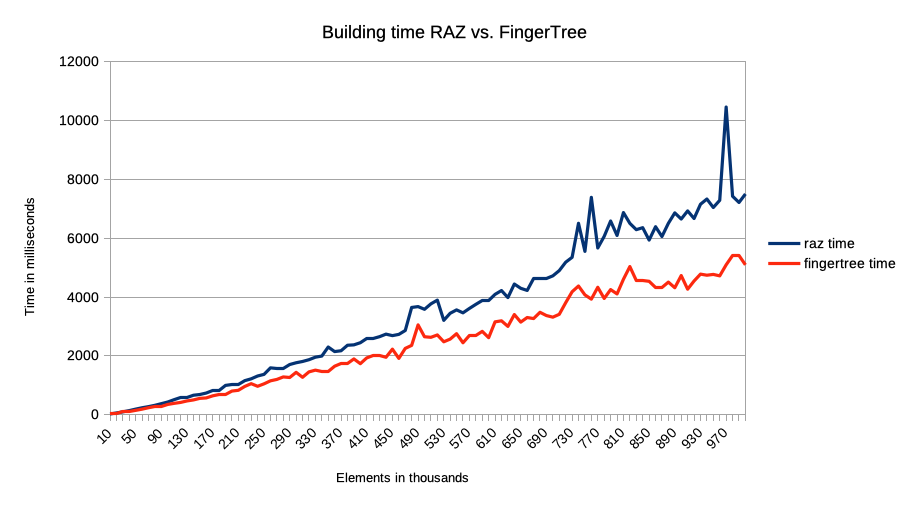
\includegraphics[width=\textwidth]{raz_ftree_exp_1}
  \captionsetup{type=figure}
  \captionof{figure}{Experiment 1 Results}
  \label{fig:raz_ftree_1}
\end{minipage}

Although this results are not completely the same, I can not conclude that the paper is wrong because the implementations from one language to other is different and internal running time also is different. This can be seen in the measure of \acrshort{ftree} which is also different.

\subsection{Experiment 2}
In this experiment a structure with $1$ Million records is built initially and $1000000$ record more is insert each time increasing the structure until reach to $100$ Million records. This is done for both \acrshort{raz} and \acrshort{ftree} and taking time in \textit{nanoseconds} on each case.

\begin{listing}[H]
  \inputminted[firstline=37, lastline=47, breaklines]{haskell}{../src/Experiments.hs}
  \caption{Extracted from source code src/Experiments.hs}
  \label{src:rac:6}
\end{listing}

The results in this case are more closer to what it was expected regarding the papers' results. This is because in the authors work the time taken by the \acrshort{raz} is worse for big amount of records rather than \acrshort{ftree}.

\begin{minipage}[t]{\linewidth}
  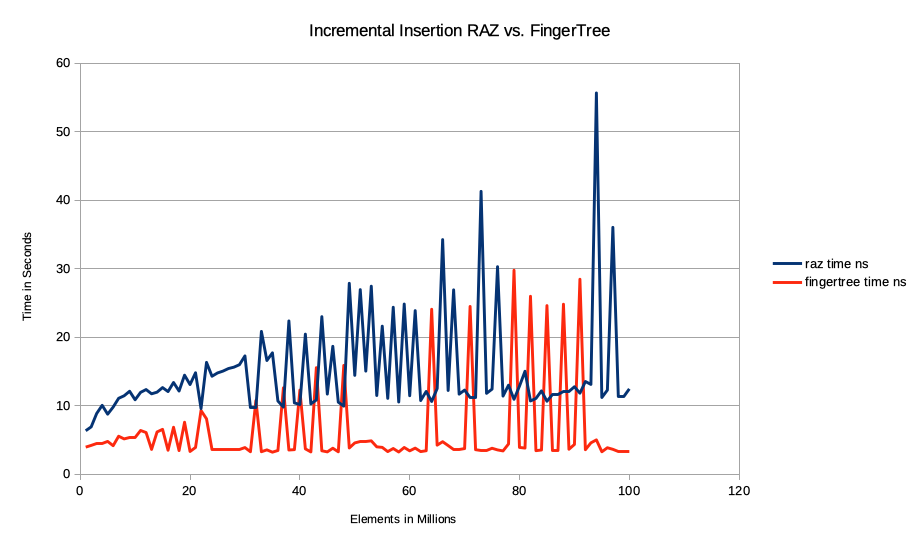
\includegraphics[width=\textwidth]{raz_ftree_exp_2}
  \captionsetup{type=figure}
  \captionof{figure}{Experiment 2 Results}
  \label{fig:raz_ftree_2}
\end{minipage}

Although this, we can see the impact of amortization on \textit{refocusing} because at some peaks, for example in $22$, $64$, $71$ millions for example times are much more better for \acrshort{raz}.

In this case I have been able to showed that amortized time in my experiments are better than in the authors experiments where it can be seen worst times in general.


\subsection{Benchmark}
As I have pointed out in the previous sections, the benchmark analysis I realized was done over the set of principal functions that provide the structure.

All the details of this report can be seen here \mintinline{bash}{../output/report_benchmark_1590325854.html} but in general we can show in the following analysis the summary results and extract some conclusions:


\begin{minipage}[t]{\linewidth}
  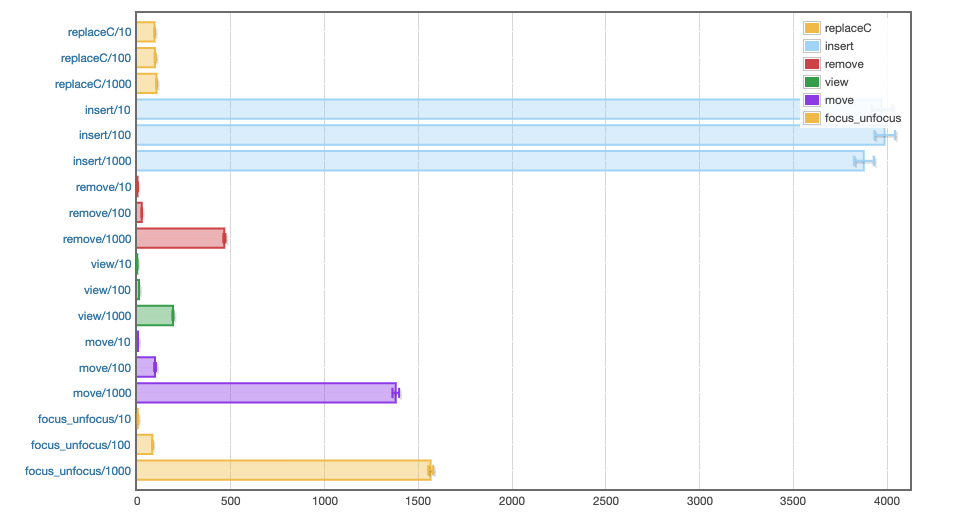
\includegraphics[width=\textwidth]{raz_bench}
  \captionsetup{type=figure}
  \captionof{figure}{Benchmark Results - Values are in Milliseconds}
  \label{fig:raz_bench}
\end{minipage}

As we can see the functions that has \textbf{amortized} $O(1)$ like \mintinline{haskell}{remove} or \mintinline{move} fluctuates when the structure increase which is expected.

Regarding functions with $O(1)$ \textbf{worst-case} like \mintinline{haskell}{view}, \mintinline{haskell}{replaceC} and \mintinline{haskell}{insert} remains constant in their running time accordingly on what it is expected too.

At last it can be also appreciate that \textbf{refocusing} also it is affected by the increase of the size as other function with amortization complexity.

\section{Conclusions}
In conclusion I think the structure behave more or less the same as the authors claimed in the paper, although I disagree a little with the purpose that is a better alternative than \acrshort{ftree}.

On the one hand, it is not conclusive the data that the authors provide in the paper and there is not enough statistical data on the experiment conducted more than the experiments that I have described on this analysis. I think that some more exhaustive experiment should be handled in order to state significant performance advantage of this structure among others.

Secondly, I think the mathematical analysis of the paper is quite poor compare with other papers of the same kind and there is also some propositions statements that have not been proved formally in a rigorous manner.

In spite of this, I believe that the claimed of the authors regarding the simplicity of the structure is true, because it allows to any \acrshort{fp} Programmer to do a similar implementation in other language in a matter of minutes. The extensibility is also another key aspect of the structure taking into consideration the \textit{List-like} approach of the combinator signatures.

Although as I have stated the implementation of the structure is easy, it is not true that optimize the structure to work under optimal conditions at least to achieve similar results as the paper, it is an easy task. Just the opposite I think that there are so much things to take into consideration and one key aspect is since the structure works with  \textit{Random Number Generators}, this could lead to worst performance as expected because the structure heavily rest on this fact for insertion. It is true that this factor only affects for building the structure or modifying it and not for manipulating and searching.

In general I believe it is a quite clever structure with a lot of work to be done for optimizing and gaining in simplicity for extension.

\bibliographystyle{alpha}
\bibliography{report}

\printglossary[type=\acronymtype]

\appendix\label{apx:org}
\section{Haskell}
\subsection{Source Code}
In the source code there are 3 folders with code:

\begin{itemize}
  \item \textbf{app}: Which contains the program source code file. Here we can find:
  \item \textbf{src}: Contains the implementation source code of \acrshort{raz}.
    \begin{itemize}
      \item \textbf{\mintinline{haskell}{src/Experiments.hs}}: It contains the different experiment run.
      \item \textbf{\mintinline{haskell}{src/Data/Zipper/Random.hs}}: \acrshort{raz} Implementation.
    \end{itemize}
  \item \textbf{test}: Contains Property based testing that automatize the test of the implemented \acrshort{raz}
\end{itemize}

\subsection{Run the Code}
All the solution has been coded with \textbf{Stack} \cite{stack} version 2.1.3 or higher. It is a prerequisite to install \textit{stack} for running this code.

\subsubsection{Running Experiments}
In order to run the experiments just do the following in each case.

\begin{itemize}
  \item \textbf{Experiment 1} Building the structure from scratch with different sizes.

\begin{minted}{bash}
stack build
stack exec raz experiment-1
\end{minted}

\setlength{\rightskip}{0pt plus 1 fil}
This is going to left the results in CSV file format under \mintinline{bash}{output/result_exp1_UNIX_TIME_IN_MILLIS.csv}.


  \item \textbf{Experiment 2} Insert 1 million elements maintaining the same structure until reach 100 Millions elements.

\begin{minted}{bash}
stack build
stack exec raz experiment-2
\end{minted}

\setlength{\rightskip}{0pt plus 1 fil}
This is going to left the results in CSV file format under \mintinline{bash}{output/result_exp2_UNIX_TIME_IN_MILLIS.csv}.

  \item \textbf{Benchmark} Benchmark general execution time for each combinator \mintinline{haskell}{insert},  \mintinline{haskell}{alter}, \mintinline{haskell}{remove}, \mintinline{haskell}{move}, \mintinline{haskell}{focus}, \mintinline{haskell}{unfocus}.

\begin{minted}{bash}
stack build
stack exec raz bench
\end{minted}

\setlength{\rightskip}{0pt plus 1 fil}
This is going to left an HTML report with the benchmark results in \mintinline{bash}{output/report_benchmark_UNIX_TIME_IN_MILLIS.html}.


\end{itemize}

\section{Generated Outputs}\label{apx:reports}
All the Generated Outputs that has been used to build this document are under \mintinline{haskell}{output} folder.

\section{Report PDF Document}
This report document is under \mintinline{haskell}{doc} folder alongside images that are embedded in this report.

\end{document}

